\begin{frame}
\frametitle{Why Modularization}
\begin{itemize}
\item Growth management
\pause
\item Software quality improvement
\pause
\item Facilitating add-ons
\pause
\item Separate third party libraries
\pause
\item Optional Components
\end{itemize}
\end{frame}

{
\setbeamertemplate{navigation symbols}{}
\setbeamertemplate{background canvas}{
  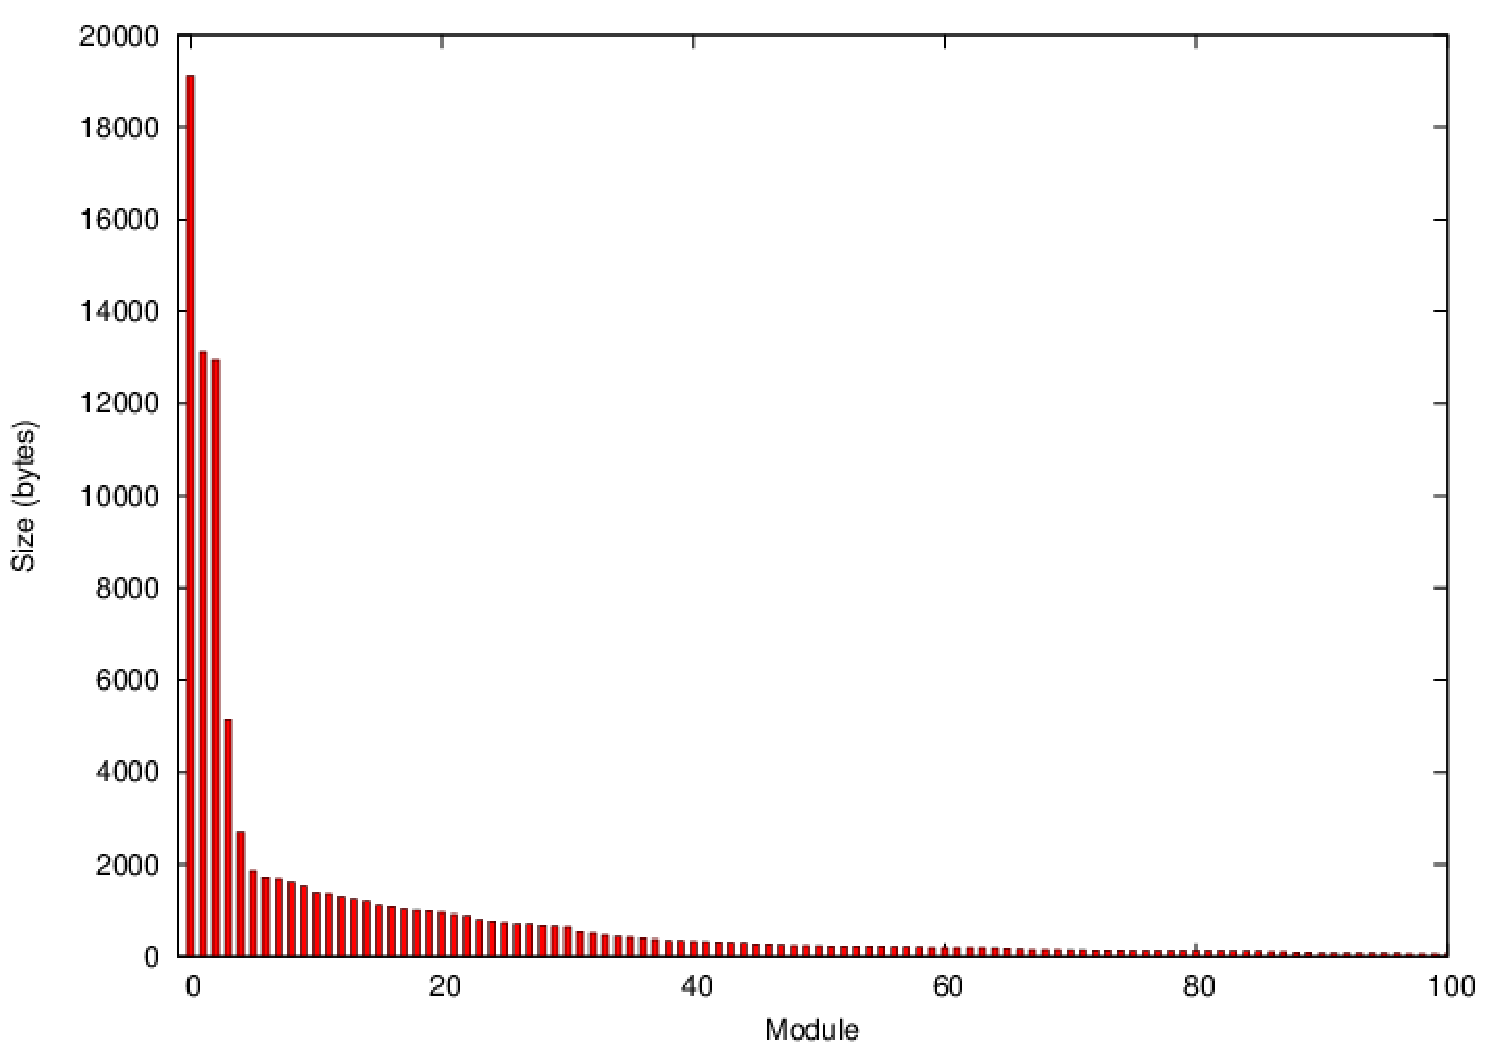
\includegraphics[width=\paperwidth,height=\paperheight]{moduleSizePlot.pdf}
}
\begin{frame}[plain]
\end{frame}
}


{
\setbeamertemplate{navigation symbols}{}
\setbeamertemplate{background canvas}{
  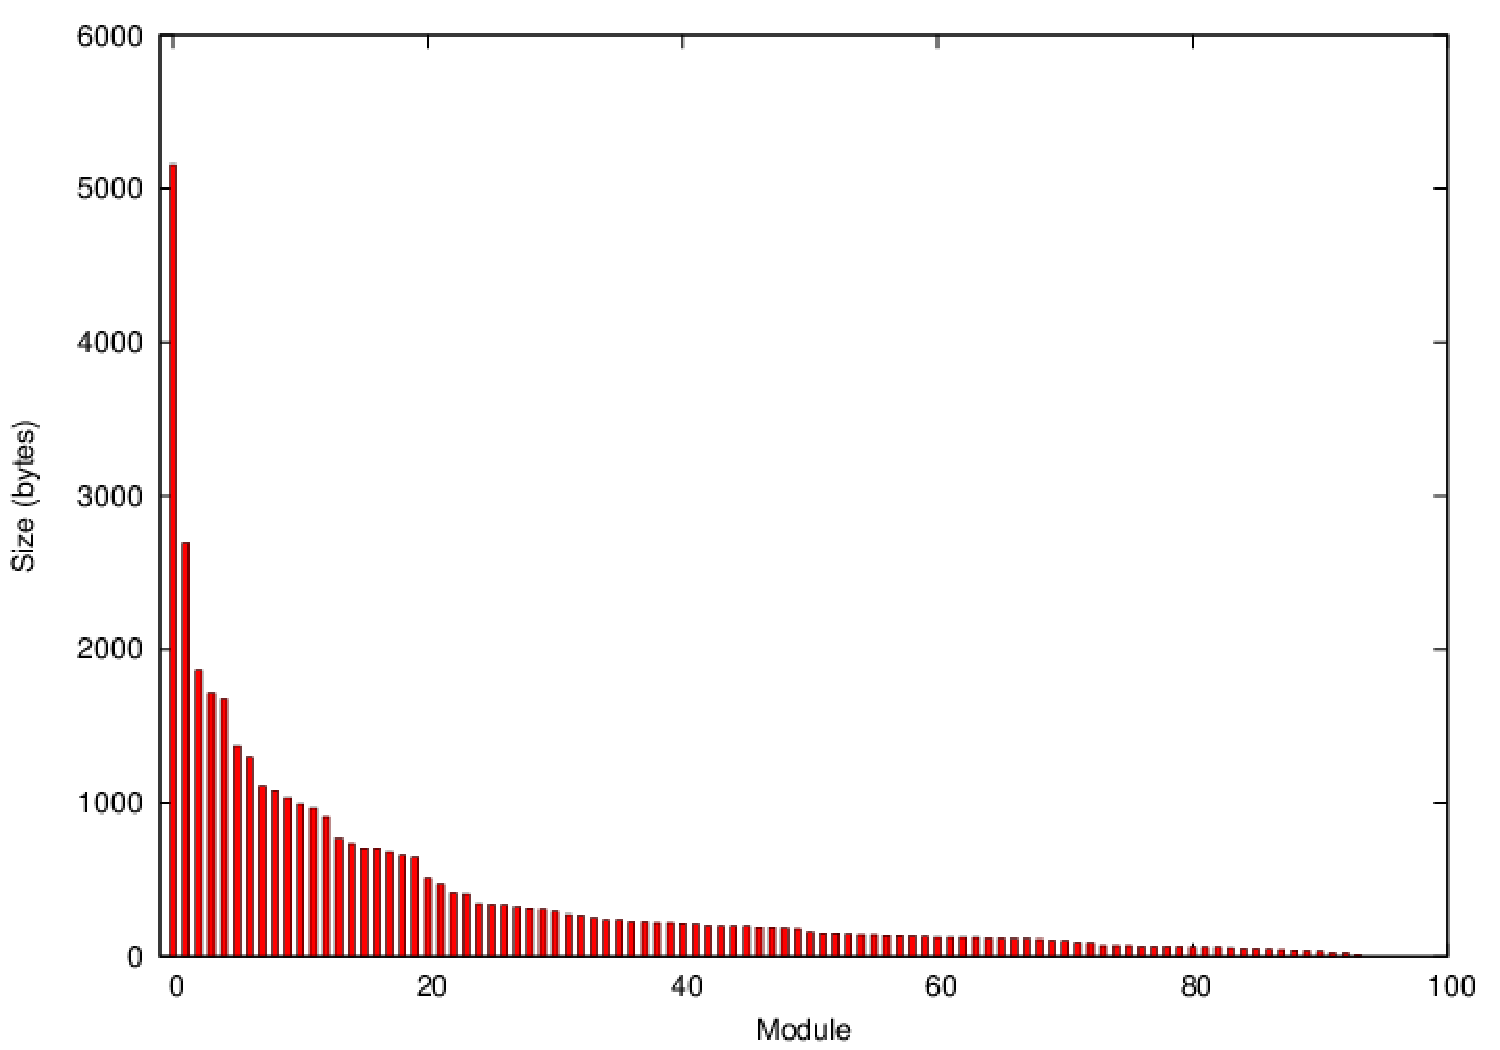
\includegraphics[height=\paperheight]{moduleSizePlotNoThirdParty.pdf}
}
\begin{frame}[plain]
\end{frame}
}


{
\setbeamertemplate{navigation symbols}{}
\setbeamertemplate{background canvas}{
  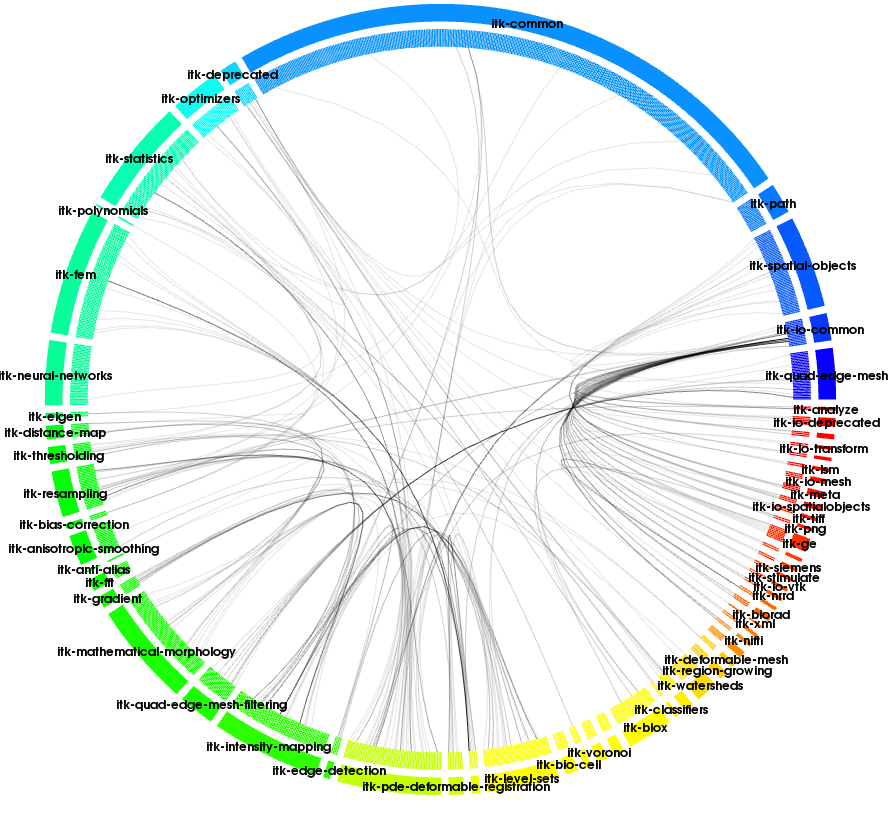
\includegraphics[height=\paperheight]{moduleDependency.png}
}
\begin{frame}[plain]
\end{frame}
}


\begin{frame}
\frametitle{ITK Module Grouping}
\begin{itemize}
\item  How many groups?
\pause
\item  Grouping criteria
\pause
\end{itemize}
\end{frame}



\begin{frame}
\frametitle{Modular darshboard }
\begin{itemize}
\item  Module-by-module dashboard submission
\pause
\item  Code coverage per module
\end{itemize}
\end{frame}


\begin{frame}
\frametitle{How to add a module into ITK}
\begin{itemize}
\item Where to put a module (categorization)
\pause
\item How to construct a module (CMake magic)
\end{itemize}
\end{frame}


\begin{frame}
\frametitle{Modularizatoin checklist}
\begin{itemize}
\item  Module categorization: module group, module name
\pause
\item  Directory hierarchy: include, test, src
\pause
\item  CMake configuration: CMakeLists.txt
\pause
\item  Module dependency: itk-module.cmake
\pause
\item  Add tests, \href{http://www.vtk.org/Wiki/ITK/Git/Develop/Data\#Workflow}{\textcolor{red}{add testing data}}
\pause
\item  Documentation
\end{itemize}
\end{frame}


\begin{frame}
\frametitle{A toy example: ITKRAT}
\begin{itemize}
\item  itkRobustAutomaticThresholdImageFilter(RAT)
\pause
\item  An external module: ITKRAT
\end{itemize}
\end{frame}

\centeredlargetext{white}{black}{
Details about ITK Modularization can be found at \href{http://www.itk.org/Wiki/ITK\_Release\_4/Modularization}{\textcolor{red}{Wiki Page}}.
}
